\chapter{The pretty bad measurement} \label{ch:PBM}

 The contents of this chapter is based on work with Caleb McIrvin and Jamie Sikora in \cite{mcirvin2024quantum}.

 The pretty good measurement (PGM) is a way to approximate the best possible measurement for the minimum error state discrimination task.
 This chapter introduces the pretty bad measurement (PBM) as an analogue for the minimum error state exclusion problem.
 We compare the performance of these measurements with the blind guessing probability.
 We observe that while PGM can perform no worse than blind guessing, PBM can perform no better than blind guessing.
 Lastly, we look at the application of the PBM for the quantum anomaly detection/avoidance problem.

 We develop the pretty bad measurement through the following steps.
 \begin{itemize}
     \item Section~\ref{sec:ch4_PBM-PGM}: We discuss the pretty good measurement (PGM).
     \item Section~\ref{sec:ch4_PBM-offsets}: We describe how we can offset a measurement using an offset parameter.
     \item Section~\ref{sec:ch4_PBM-PBM}: We define the pretty bad measurement (PBM) as the counterpart of PGM for the quantum state exclusion problem.
     \item Section~\ref{sec:ch4_PBM-interpret}: We discuss an interpretation of PBM as PGM in a different setting.
     \item Section~\ref{sec:ch4_PBM-eg}: We illustrate an example of a state for which the PGM achieves the optimal probability for state discrimination while the PBM is a decent approximation to the optimal probability for state exclusion.
     \item Section~\ref{sec:ch4_PBM-sim}: We describe how PGM performs no worse than blind guessing and PBM performs no better than blind guessing on randomly generated examples.
     \item Section~\ref{sec:ch4_PBM-anomaly}: We discuss how PBM can be applied to the quantum anomaly detection problem.
 \end{itemize}

%%%%%%%%%%%%%%%%%%%%%%%%%%%%%%%%%%%%%%%%%%%%%%%%%%%%%%%%%%%%%%%%%%%%%%%%%%%%%%%%%%%%%%%%%%%%%%%%%%%%%%%%%%%%%%%%%%%%%%%%%%%%%%%%%%%
\section{The pretty good measurement (PGM)} \label{sec:ch4_PBM-PGM}
%%%%%%%%%%%%%%%%%%%%%%%%%%%%%%%%%%%%%%%%%%%%%%%%%%%%%%%%%%%%%%%%%%%%%%%%%%%%%%%%%%%%%%%%%%%%%%%%%%%%%%%%%%%%%%%%%%%%%%%%%%%%%%%%%%%

For an ensemble $\{(p_i,\rho_i): i \in [N]\}$, the pretty good measurement (PGM), also known as the square root measurement, introduced by Hausladen and Wootters~\cite{hausladen1994pretty} and further analyzed by Barnum and Knill~\cite{barnum2002reversing}, are the measurements $\{G_1, \dots, G_N\}$, where each operator is defined as  
\begin{equation}
    \label{eq:ch4_PBM-PGM_ops}
    G_i = P^{-1/2} \bigg( p_i \rho_i \bigg) P^{-1/2} \; \text{ where } \; 
    P = \sum_{i=1}^N p_i \rho_i.
\end{equation} 
If Bob uses the PGM for quantum state discrimination, his success probability is
\begin{align} 
\PPGM 
& = \sum_{i=1}^N p_i \inner{G_i}{\rho_i} = \sum_{i=1}^N p_i^2 \tr(P^{-1/2} \rho_i P^{-1/2} \rho_i). \label{eq:ch4_PBM-P_PGM} 
\end{align}

Barnum and Knill~\cite{barnum2002reversing} gave the following bound on the performance of the PGM.

\begin{theorem}[Barnum-Knill Inequality \cite{barnum2002reversing}]
    \label{thm:ch4_PBM-barnum-knill}
    Let $\Pbest$ denote the optimal success probability (Eq.~\eqref{eq:ch4_PBM-P_best}), then
    \begin{equation}
        \Pbest^2 \leq \PPGM \leq \Pbest.
    \end{equation}
\end{theorem} 

This bound ensures that the PGM always achieves a success probability at least as large as the square of the optimal probability, guaranteeing near-optimal performance. 

We now present a theorem which compares $\PPGM$ to the blind guessing probability, i.e., $1/N$. 
%To the best of our knowledge, comparing $\PPGM$ to the blind guessing probability, i.e., $1/k$, is not known except in trivial cases. 
%This brings us to our first main result (which we prove in the appendix). 

\begin{theorem}{\cite{renes2017better}} \label{thm:ch4_PBM-PGM}
For any set of states $\{ \rho_1, \ldots, \rho_N \}$ and probability distribution $\{ p_1, \ldots, p_N \}$, we have 
\begin{equation} 
\PPGM \geq \frac{1}{N} + \frac{(1 - N \Pbest)^2}{N (N - 1)} 
\end{equation}
where $1/N$ can be interpreted as the blind guessing probability. 
Moreover, if $\PPGM = 1/N$, then we have $\rho_i = \rho_j$ and $p_i = p_j = 1/N$ for all $i \neq j$. 
\end{theorem} 

%We prove a slightly weaker version of this theorem in Section~\ref{sec:ch4_PBM-thm_1_pf} using the concept of \emph{offsets}, discussed in the next section.

We now discuss our first step towards defining a pretty bad measurement. 

%%%%%%%%%%%%%%%%%%%%%%%%%%%%%%%%%%%%%%%%%%%%%%%%%%%%%%%%%%%%%%%%%%%%%%%%%%%%%%%%%%%%%%%%%%%%%%%%%%%%%%%%%%%%%%%%%%%%%%%%%%%%%%%%%%%
\section{Purposely messing up measurements with offsets} \label{sec:ch4_PBM-offsets}
%%%%%%%%%%%%%%%%%%%%%%%%%%%%%%%%%%%%%%%%%%%%%%%%%%%%%%%%%%%%%%%%%%%%%%%%%%%%%%%%%%%%%%%%%%%%%%%%%%%%%%%%%%%%%%%%%%%%%%%%%%%%%%%%%%%

Suppose that one is given a decent measurement for state discrimination and one wishes to make it perform worse. 
Then one way to do this is to take the outcome of this measurement and \emph{change the answer}. 
To this end, suppose we start with measurements $\{M_1, \ldots, M_N\}$ and an \emph{offset parameter} $s$. 
We define the offset measurement $\{M^s_1, \ldots, M^s_N\}$ as 
\begin{equation} 
M^s_i = M_{i \oplus s} 
\end{equation} 
where we use the notation $\oplus$ to denote cyclic addition, e.g., $5 \oplus 1 = 1$ when $N = 5$. 
Conceptually, an offset should mess up a good measurement and, conversely, could have the ability to improve a bad measurement. 
We have the need to quantify how well these offset measurements perform, thus we define 
\begin{equation} 
\alpha_s = \sum_{i=1}^N p_i \inner{M^s_i}{\rho_i} = \sum_{i=1}^N p_i \inner{M_{i \oplus s}}{\rho_i}.  
\end{equation} 
It turns out that all of these quantities are related to each other via the equality 
\begin{equation}\label{eq:ch4_PBM-EqA3} 
\sum_{s=0}^{N-1} \alpha_s = 1 
\end{equation} 
which is easily seen by noting that, for any fixed $i$, $\{M_i, M_{i \oplus 1}, \ldots, M_{i \oplus (N-1)}\}$ yields a valid POVM, and thus $\sum_{s=0}^{N-1} M_{i \oplus s} = \id$.

We now prove a slightly weaker version of Theorem~\ref{thm:ch4_PBM-PGM}.

%%%%%%%%%%%%%%%%%%%%%%%%%%%%%%%%%%%%%%%%%%%%%%%%%%%%%%%%%%%%%%%%%%%%%%%%%%%%%%%%%%%%%%%%%%%%%%%%%%%%%%%%%%%%%%%%%%%%%%%%%%%%%%%%%%%

\subsection{Proof of a slightly weaker version of Theorem~\ref{thm:ch4_PBM-PGM}} \label{ss:ch4_PBM-thm_pf}

Given the quantum states $\{\rho_1, \ldots, \rho_N\}$ and the probability distribution $\{ p_1, \ldots, p_N \}$,  
define $P = \sum_{i=1}^N p_i \rho_i$ and the measurements $\{G_1, \ldots, G_N\}$ where $G_i = P^{-1/2} \left( p_i \rho_i \right) P^{-1/2}$ as in Eq.~\eqref{eq:ch4_PBM-PGM_ops}. 
Moreover, define the $N$-dimensional vector $r$ where 
\begin{equation} 
r_i = \| P^{-1/4} \left( p_i \rho_i \right) P^{-1/4}\|_F.  
\end{equation} 
The proof begins as follows. 
First, we establish that $\PPGM = \| r \|_2^2$. 
Second, we bound $\| r \|_1 \geq 1$. 
Then showing $\PPGM \geq 1/N$ follows by Cauchy-Schwarz.  

%\bigskip 

To see that $\| r \|_2^2 = \PPGM$, we have 
\begin{equation}
    \begin{aligned} 
        \| r \|_2^2 
        & = \sum_{i=1}^N r_i^2 
        = \sum_{i=1}^N \| P^{-1/4} \left( p_i \rho_i \right) P^{-1/4} \|_F^2
        = \sum_{i=1}^N \tr \left( P^{-1/4} \left( p_i \rho_i \right) P^{-1/2} \left( p_i \rho_i \right) P^{-1/4} \right) \\
        & = \sum_{i=1}^N p_i \ \tr \left( \rho_i \ P^{-1/2} \left( p_i \rho_i \right) \ P^{-1/2} \right)
        = \sum_{i=1}^N p_i \ \tr \left( \rho_i G_i \right)
        = \PPGM.  
    \end{aligned}
\end{equation} 

We now bound the following quantity:  
\begin{equation}
    \begin{aligned} 
        p_i \ \inner{G_{i \oplus s}}{\rho_i}
        & = p_i \ \tr( P^{-1/2} (p_{i \oplus s} \rho_{i \oplus s})\ P^{-1/2} \ \rho_i ) \\
        & = \tr\left( P^{-1/4} \left( p_{i \oplus s} \rho_{i \oplus s} \right) P^{-1/4} P^{-1/4} \left( p_i \rho_i \right) P^{-1/4} \right) \\ 
        & \leq \| P^{-1/4} \left( p_{i \oplus s} \rho_{i \oplus s} \right) P^{-1/4} \|_F \|  P^{-1/4} \left( p_i \rho_i \right) P^{-1/4} \|_F \label{eq:ch4_PBM-temp} \\ 
        & = r_{i \oplus s} \cdot r_i. 
    \end{aligned}
\end{equation}

This bound is useful in showing $1 \leq \| r \|_1$. 
Using Eq.~\eqref{eq:ch4_PBM-EqA3}, we have 
\begin{equation}
    \begin{aligned}
        1 = \sum_{s=0}^{N-1} \alpha_s & = \sum_{s=0}^{N-1} \sum_{i=1}^N p_i \ \inner{G_{i \oplus s}}{\rho_i}
         \leq \sum_{s=0}^{N-1} \sum_{i=1}^N r_{i \oplus s} \cdot r_i
         = \left( \sum_{i=1}^N r_i \right)^2 
         = \| r \|_1^2 
    \end{aligned} 
\end{equation}
noting the last equality holds since $r_i \geq 0$ for all $i$. 

%\bigskip 

Let $e$ be the $N$-dimensional all-ones vector and note that $\| r \|_1 = \inner{r}{e}$. 
Then by the Cauchy-Schwarz inequality (for vectors), we have 
\begin{equation} \label{eq:ch4_PBM-lastline}
1 \leq \| r \|_1 = \inner{r}{e} \leq \| r \|_2 \| e \|_2 = \sqrt{\PPGM} \cdot \sqrt{N} 
\end{equation} 
proving that $\PPGM \geq 1/N$.%, as desired. 

%\bigskip

Now, if we have that $\PPGM = 1/N$, we must have equality throughout~\eqref{eq:ch4_PBM-lastline}. 
This means that the vector $r$ must be proportional to $e$ and $\| r \|_1 = 1$. 
These together imply that $r_i = 1/N$ for all $i$ which further implies that $P^{-1/4} (p_i \rho_i) P^{-1/4} \neq 0$ for all $i$, as well as $p_i \neq 0$ for all $i$. 

We further require inequality Eq.~\eqref{eq:ch4_PBM-temp} to hold with equality, i.e., we must saturate Cauchy-Schwarz \emph{at every $i$ and $i \oplus s$}. 
This can only be true if there exists $\lambda_{i,j} \neq 0$ such that 
\begin{align}
    P^{-1/4} (p_i \rho_i) P^{-1/4} = \lambda_{i,j} P^{-1/4} (p_{j} \rho_{j}) P^{-1/4}   
\end{align} 
for all $i$ and $j$. 
Multiplying both sides by $P^{1/4}$, we have 
\begin{align} \label{thanos}
    p_i \rho_i = \lambda_{i,j} p_{j} \rho_{j}. 
\end{align} 
Taking the trace of both sides, we get 
\begin{align}
    \lambda_{i,j} = \frac{p_i}{p_j}. 
\end{align} 
From Eq.~\eqref{thanos}, we have $\rho_i = \rho_j$ for all $i$ and $j$. 

All that remains to prove is that $p_i = 1/N$  for all $i$. 
Recall that $r_i = 1/N$ for all $i$. 
Thus, we have 
\begin{align} 
1
 = \frac{r_i}{r_j} 
 = \frac{\| P^{-1/4} (p_i \rho_i) P^{-1/4} \|_F}{\| P^{-1/4} (p_j \rho_j) P^{-1/4} \|_F} 
 = \frac{p_i}{p_j} \frac{\| P^{-1/4} \rho_i P^{-1/4} \|_F}{\| P^{-1/4} \rho_j P^{-1/4} \|_F} 
 = \frac{p_i}{p_j} 
\end{align}  
where the last equality holds since $\rho_i = \rho_j$ for all $i$ and $j$. 
Thus, $p_i = 1/N$ for all $i$, as required.

%%%%%%%%%%%%%%%%%%%%%%%%%%%%%%%%%%%%%%%%%%%%%%%%%%%%%%%%%%%%%%%%%%%%%%%%%%%%%%%%%%%%%%%%%%%%%%%%%%%%%%%%%%%%%%%%%%%%%%%%%%%%%%%%%%%
\section{The pretty bad measurement (PBM)} \label{sec:ch4_PBM-PBM}
%%%%%%%%%%%%%%%%%%%%%%%%%%%%%%%%%%%%%%%%%%%%%%%%%%%%%%%%%%%%%%%%%%%%%%%%%%%%%%%%%%%%%%%%%%%%%%%%%%%%%%%%%%%%%%%%%%%%%%%%%%%%%%%%%%%

We now define the counterpart to the PGM which now approximates $\Pworst$ instead. 
Our approach is quite simple and borrows much of the elegance from the PGM. 
We define it below and then give some interpretations of it. 
\begin{definition} 
Let $\{G_1, \ldots, G_N\}$ be the pretty good measurement. 
The pretty bad measurement (PBM) is defined as the POVM $\{B_1, \ldots, B_N\}$ where 
\begin{equation} 
B_i = \frac{1}{N-1} \bigg( \id - G_i \bigg).  
\end{equation} 
\end{definition} 

One way to interpret the PBM is by viewing it as the PGM with a uniformly random offset. 
In other words, 
\begin{align} 
B_i & = \frac{1}{N-1} \sum_{s=1}^{N-1} G^s_i 
\end{align} 
noting that we omit the $s=0$ index since $G_i^0 = G_i$.  
With this, we can calculate the success probability of the PBM as 
\begin{align} 
\PPBM 
= \sum_{i=1}^N p_i \, \tr(\rho_i B_i)
= \frac{1}{N-1} \sum_{s=1}^{N-1} \sum_{i=1}^N p_i \tr(\rho_i G^s_i)
= \frac{1}{N-1} \sum_{s=1}^{N-1} \alpha_s. \label{eq:ch4_PBM-JohnWick}
\end{align} 
Since $\alpha_0 = \PPGM$, as this is the no-offset success probability, we have the following equation which follows directly from Eq.~\eqref{eq:ch4_PBM-EqA3}  
\begin{equation}
\PPGM + (N-1) \PPBM = 1. \label{eq:ch4_PBM-PGM_PBM} 
\end{equation} 

By combining with Theorem~\ref{thm:ch4_PBM-PGM}, we have our main result, below, which is the counterpart to the PGM bound, Theorem~\ref{thm:ch4_PBM-PGM}. 

\begin{theorem} \label{thm:ch4_PBM-PBM}
For any set of states $\{ \rho_1, \ldots, \rho_N \}$ and probability distribution $\{ p_1, \ldots, p_N \}$, we have 
\begin{equation} 
\PPBM \leq \frac{1}{N} - \frac{(1 - N \Pbest)^2}{N (N - 1)^2}. 
\end{equation} 
Moreover, if $\PPBM = 1/N$, then we have $\rho_i = \rho_j$ and $p_i = p_j = 1/N$ for all $i \neq j$. 
\end{theorem} 

As a consequence of our discussion so far, we have 
\begin{equation}
\Pbest \geq \PPGM \geq \frac{1}{N} \geq \PPBM \geq \Pworst.
\label{eq:ch4_PBM-AllInequalities}
\end{equation} 

%%%%%%%%%%%%%%%%%%%%%%%%%%%%%%%%%%%%%%%%%%%%%%%%%%%%%%%%%%%%%%%%%%%%%%%%%%%%%%%%%%%%%%%%%%%%%%%%%%%%%%%%%%%%%%%%%%%%%%%%%%%%%%%%%%%
\section{Another interpretation} \label{sec:ch4_PBM-interpret}
%%%%%%%%%%%%%%%%%%%%%%%%%%%%%%%%%%%%%%%%%%%%%%%%%%%%%%%%%%%%%%%%%%%%%%%%%%%%%%%%%%%%%%%%%%%%%%%%%%%%%%%%%%%%%%%%%%%%%%%%%%%%%%%%%%%

There is another way to interpret the PBM which is as the PGM \emph{in a different setting}.  
For the set of states 
$\{ \rho_1, \ldots, \rho_N \}$ with probabilities 
$\{ p_1, \ldots, p_N \}$, define a new problem instance 
$\{ \wt{\rho}_1, \ldots, \wt{\rho}_N \}$ with probabilities 
$\{ \wt{p}_1, \ldots, \wt{p}_N \}$ 
where 
\begin{equation} 
\wt{\rho}_i 
= \frac{1}{1-p_i} \sum_{j \neq i} p_j \rho_j 
\quad \text{ and } \quad
\wt{p}_i 
= \frac{1-p_i}{N-1} 
\end{equation} 
assuming $p_i \neq 1$ for all $i$. 
We can think of $\wt{\rho}_i$ as averaging over all of the $\rho_j$s with different indices. 
Thus, by guessing $i$ accurately in the tilde setting one is actually guessing poorly in the original setting.  
Before analyzing the PGM in the tilde setting, notice that 
\begin{equation}
\wt{p}_i \wt{\rho}_i 
= \frac{1}{N-1} \sum_{j \neq i} p_j \rho_j 
= \frac{1}{N-1} (P - p_i \rho_i)  
\end{equation}
recalling the definition of $P$ from Eq.~\eqref{eq:ch4_PBM-PGM_ops}. 
%From here, we have 
We also have that 
%\begin{equation}
$\wt{P} 
= \sum_{i=1}^N \wt{p}_i \wt{\rho}_i 
= P$.   
%\end{equation}
Denoting the PGM in the tilde setting as $\{ \wt{G}_1, \ldots, \wt{G}_N \}$, we can calculate that   
\begin{equation*} 
\wt{G}_i 
= \wt{P}^{-1/2} \bigg( \wt{p}_i \wt{\rho}_i \bigg) \wt{P}^{-1/2}   
= B_i. 
\end{equation*}
Thus, one can view the PBM as the PGM if the problem instance is changed accordingly.  

%\smallskip 
\paragraph{Remark.} We note that the mixing of POVM elements considered above is studied more generally in the context of \emph{reverse channels} and \emph{reverse observables}
which have been used in the study of compatibility~\cite{filippov2017necessary}.  

%%%%%%%%%%%%%%%%%%%%%%%%%%%%%%%%%%%%%%%%%%%%%%%%%%%%%%%%%%%%%%%%%%%%%%%%%%%%%%%%%%%%%%%%%%%%%%%%%%%%%%%%%%%%%%%%%%%%%%%%%%%%%%%%%%%
\section{Illustrative examples} \label{sec:ch4_PBM-eg}
%%%%%%%%%%%%%%%%%%%%%%%%%%%%%%%%%%%%%%%%%%%%%%%%%%%%%%%%%%%%%%%%%%%%%%%%%%%%%%%%%%%%%%%%%%%%%%%%%%%%%%%%%%%%%%%%%%%%%%%%%%%%%%%%%%%

Consider the three trine states, defined as 
\begin{equation}
    \begin{aligned} 
        \ket{\psi_1} = \ket{0}, &\quad
        \ket{\psi_2} = \cos(2\pi/3) \ket{0} + \sin(2\pi/3) \ket{1}, \\
        \ket{\psi_3} &= \cos(4\pi/3) \ket{0} + \sin(4\pi/3) \ket{1}. 
    \end{aligned} 
\end{equation}
These are shown in Fig.~\ref{fig:ch4_PBM-trine}, along with the five quantities of interest.

\begin{comment}
\begin{figure}[h]
    \centering
    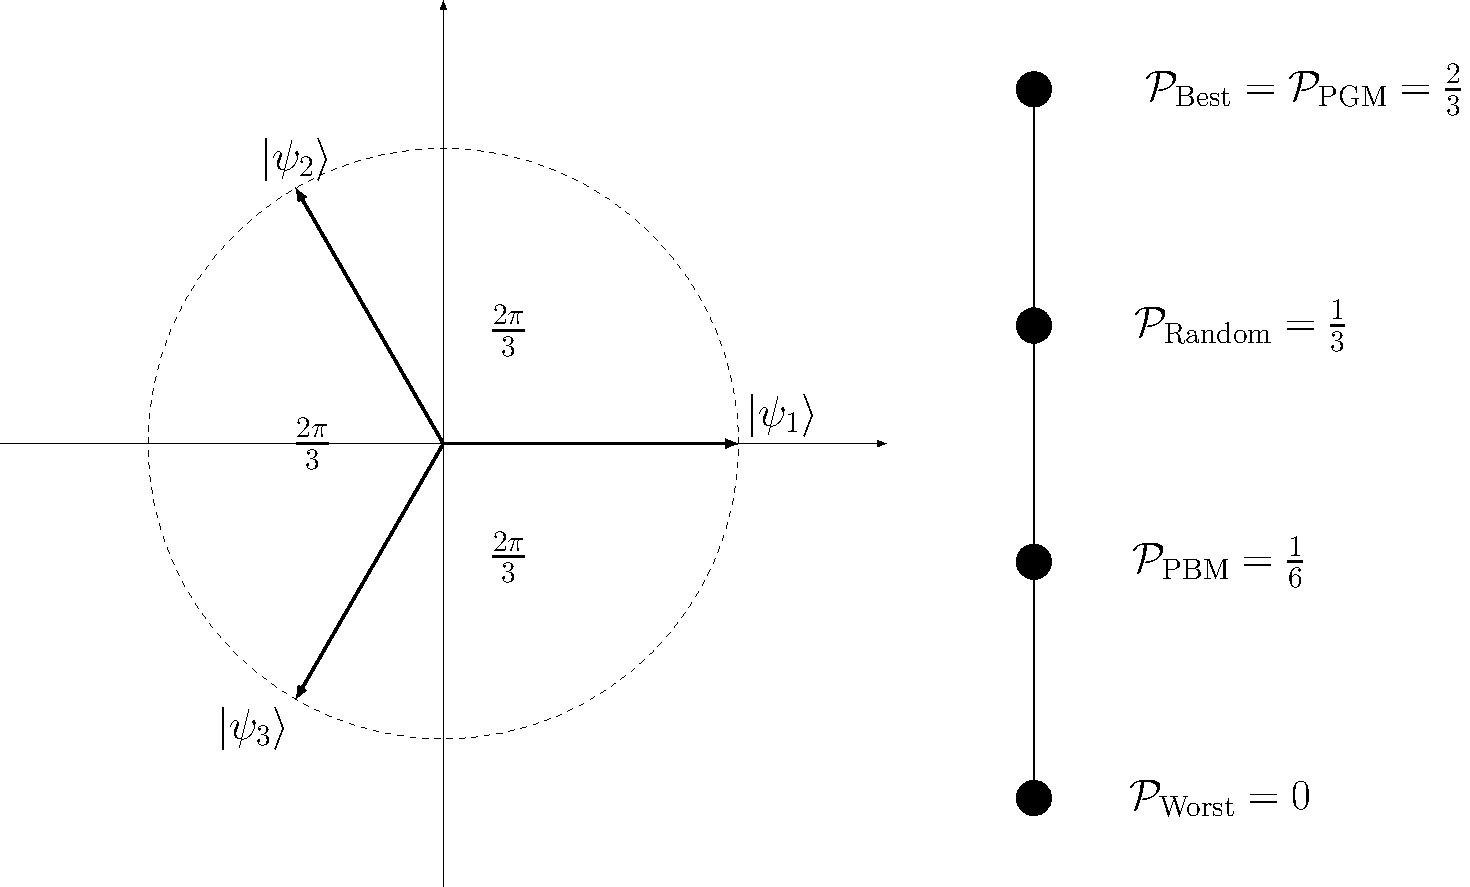
\includegraphics[scale=0.5]{figs/ch4_PBM/trine_states.pdf}
    \caption{If given a trine state, each with equal probability, we have $\Pbest = \PPGM = 2/3$, 
    $\mathcal{P}_{\text{Random}} = 1/3$ being the blind guessing probability, and $\PPBM = 1/6$ approximating $\Pworst = 0$. 
    The pretty good measurement is given by the POVM $G_i = \frac{2}{3} \kb{\psi_i}$,
    the pretty bad measurement is given by the POVM $B_i = \frac{1}{3} \sum_{j \neq i} \kb{\psi_j}$,
    and the worst measurement is given by $W_i = \frac{2}{3} \kb{\psi_i^{\perp}}$, where $\kb{\psi_i^{\perp}}$ is a $\pi/2$-rotation of $\ket{\psi_i}$.}
    \label{fig:ch4_PBM-trine}
\end{figure}
\end{comment}

\begin{figure}[h]
    \centering
    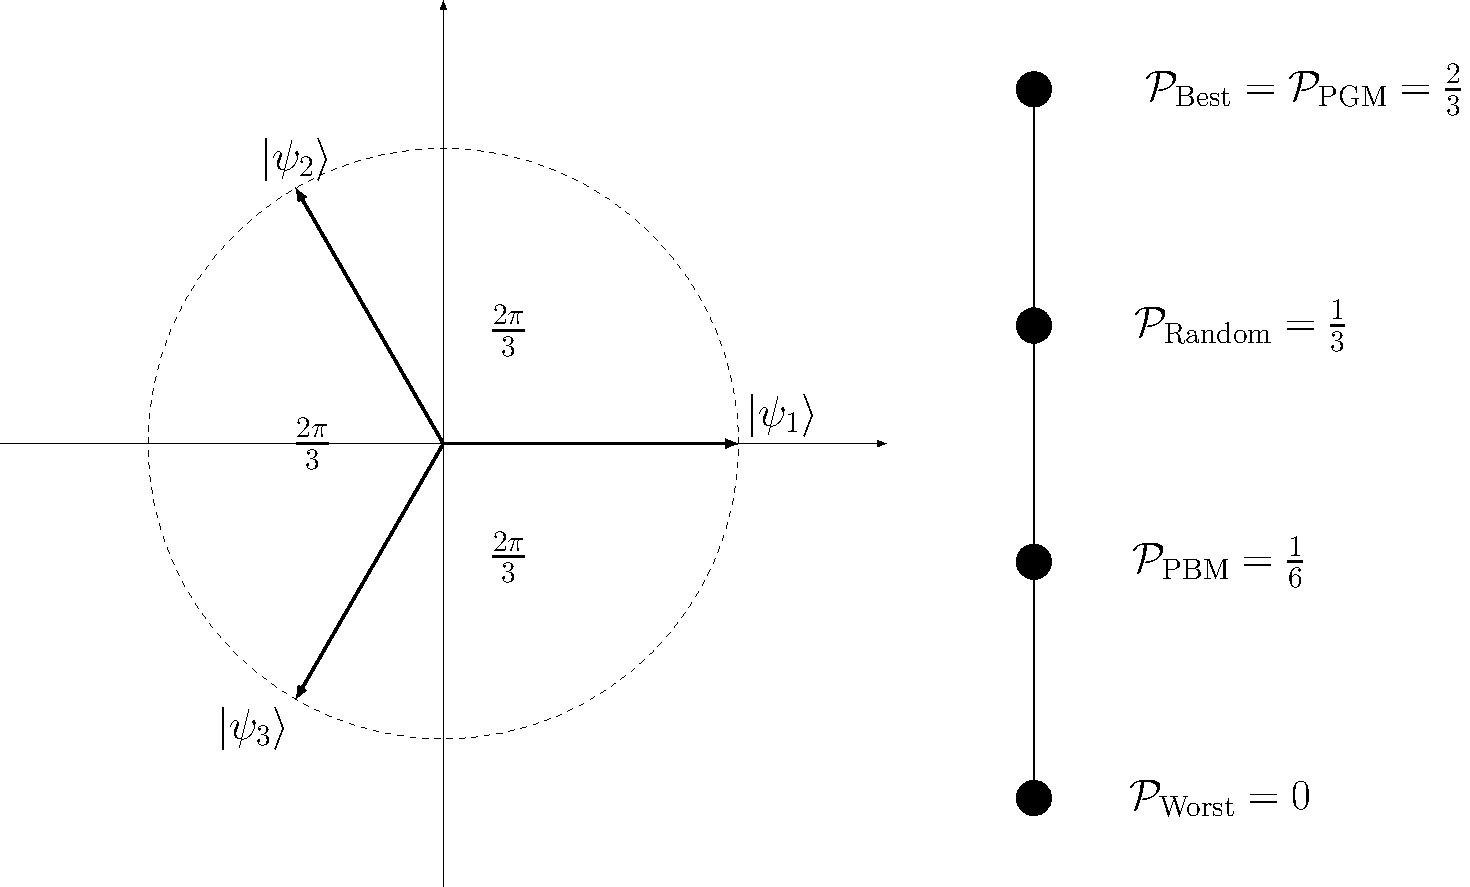
\includegraphics[
        scale=0.5,
        alt={
            Diagram illustrating three equally likely trine qubit states, labeled psi one, psi two, and psi three. 
            The states are symmetrically arranged, with equal angular separation. 
            The figure also illustrates the measurement directions associated with the pretty good, pretty bad, and worst measurements. 
            The pretty good measurement is aligned with each corresponding trine state. 
            The pretty bad measurement outcome associated with a state is formed from the other two trine states. 
            The worst measurement is aligned with the state orthogonal to each corresponding trine state.
        }
    ]{figs/ch4_PBM/trine_states.pdf}

    \caption{
        If given a trine state, each with equal probability, we have $\Pbest=\PPGM=2/3$, with $\mathcal{P}_{\text{Random}}=1/3$ being the blind-guessing probability, and $\PPBM=1/6$ approximating $\Pworst=0$.
        The pretty good measurement is given by the POVM $G_i=\frac{2}{3}\kb{\psi_i}$; the pretty bad measurement is given by the POVM $B_i=\frac{1}{3}\sum_{j\neq i}\kb{\psi_j}$; and the worst measurement is given by $W_i=\frac{2}{3}\kb{\psi_i^{\perp}}$, where $\kb{\psi_i^{\perp}}$ is a $\pi/2$ rotation of $\ket{\psi_i}$.
    }
    \label{fig:ch4_PBM-trine}
\end{figure}

We remark that this example sees the PGM being a perfect approximation of $\Pbest$ while the PBM is a decent, but not perfect, approximation of $\Pworst$. 
It is an interesting question to see in which cases the PBM is the worst measurement. 
The above example suggests that this is indeed tricky to answer since it does not coincide with the settings where the PGM is the best measurement. 
 
If the set of states is antidistinguishable, that is, if ${\Pworst = 0}$, then if $\PPBM = \Pworst$, then by Eq.~\eqref{eq:ch4_PBM-PGM_PBM}, we must have $\PPGM = 1$.  
In this case, the states must have orthogonal supports and we have 
\begin{equation} 
\Pbest = \PPGM = 1 \; \text{ and } \; \PPBM = \Pworst = 0. 
\end{equation} 

On the other hand, if the set of states is maximally indistinguishable, i.e., $\rho_i = \rho_j$ and $p_i = p_j = 1/N$, for all $i \neq j$, then we have 
\begin{equation} \label{eq:ch4_PBM-allthesame}
    \Pbest = \PPGM = \frac{1}{N} = \PPBM = \Pworst. 
\end{equation} 
What is interesting in the above two examples is that PBM being the worst measurement implies that PGM is the best measurement. 
This is actually true in general, which we state below% and prove in the appendix
, however the trine state example shows that the converse is not true. 

\begin{lemma}
If $\PPBM = \Pworst$, then $\PPGM = \Pbest$.  
\end{lemma} 
\begin{proof}
Suppose $\PPBM = \Pworst$. 
Consider the \emph{best} measurement $\{ M_1, \ldots, M_N \}$ and its random offset measurement probabilities $\alpha_s$. 
With this, we have $\alpha_0 = \Pbest$ and note that $\alpha_s \geq \Pworst = \PPBM$ for all $s$. 
By Eq.~\eqref{eq:ch4_PBM-EqA3} we get
\begin{align}
1 
 = \sum_{s = 0}^{N-1} \alpha_s 
 = \Pbest + \sum_{s = 1}^{N-1} \alpha_s 
 \geq \Pbest + \sum_{s = 1}^{N-1} \PPBM 
 \geq \PPGM + (N-1) \PPBM 
 = 1  
\end{align}
where the last equality holds by Eq.~\eqref{eq:ch4_PBM-PGM_PBM}. 
Thus, we have equality throughout, proving that $\PPGM = \Pbest$.
\end{proof}

%%%%%%%%%%%%%%%%%%%%%%%%%%%%%%%%%%%%%%%%%%%%%%%%%%%%%%%%%%%%%%%%%%%%%%%%%%%%%%%%%%%%%%%%%%%%%%%%%%%%%%%%%%%%%%%%%%%%%%%%%%%%%%%%%%%
\section{Numerical simulations} \label{sec:ch4_PBM-sim}
%%%%%%%%%%%%%%%%%%%%%%%%%%%%%%%%%%%%%%%%%%%%%%%%%%%%%%%%%%%%%%%%%%%%%%%%%%%%%%%%%%%%%%%%%%%%%%%%%%%%%%%%%%%%%%%%%%%%%%%%%%%%%%%%%%%

We have discussed how the PGM always performs no worse than blind guessing and consequently proved that the PBM always performs no better than blind guessing.
To get a better idea of how these two probabilities compare, we calculate them on many randomly generated examples. 
To generate random states, we can use the Bloch sphere to define a parameterized qubit $\rho(\theta, \phi)$ as 
\begin{equation*}
    \rho(\theta, \phi) = \frac{1}{2} \mathds{1} + \frac{\sin(\theta)\cos(\phi)}{2} X + \frac{\sin(\theta)\sin(\phi)}{2}Y + \frac{\cos(\theta)}{2}Z 
\end{equation*}
where $X$, $Y$, and $Z$ are the Pauli operators and ${\theta, \phi \in (0, 2\pi)}$ are real parameters which we randomly generate. 
We generate $1000$ random qubit instances $\{ \rho_1, \ldots, \rho_N \}$ for $N=2$ in Fig.~\ref{fig:ch4_PBM-pgm_vs_pbm_two_states} and for $N=6$ in Fig.~\ref{fig:ch4_PBM-pgm_vs_pbm_six_states}, each with randomly generated probabilities $(p_1, \ldots, p_N)$. % as well.  

\begin{comment}
\begin{figure}[h]
    \centering
    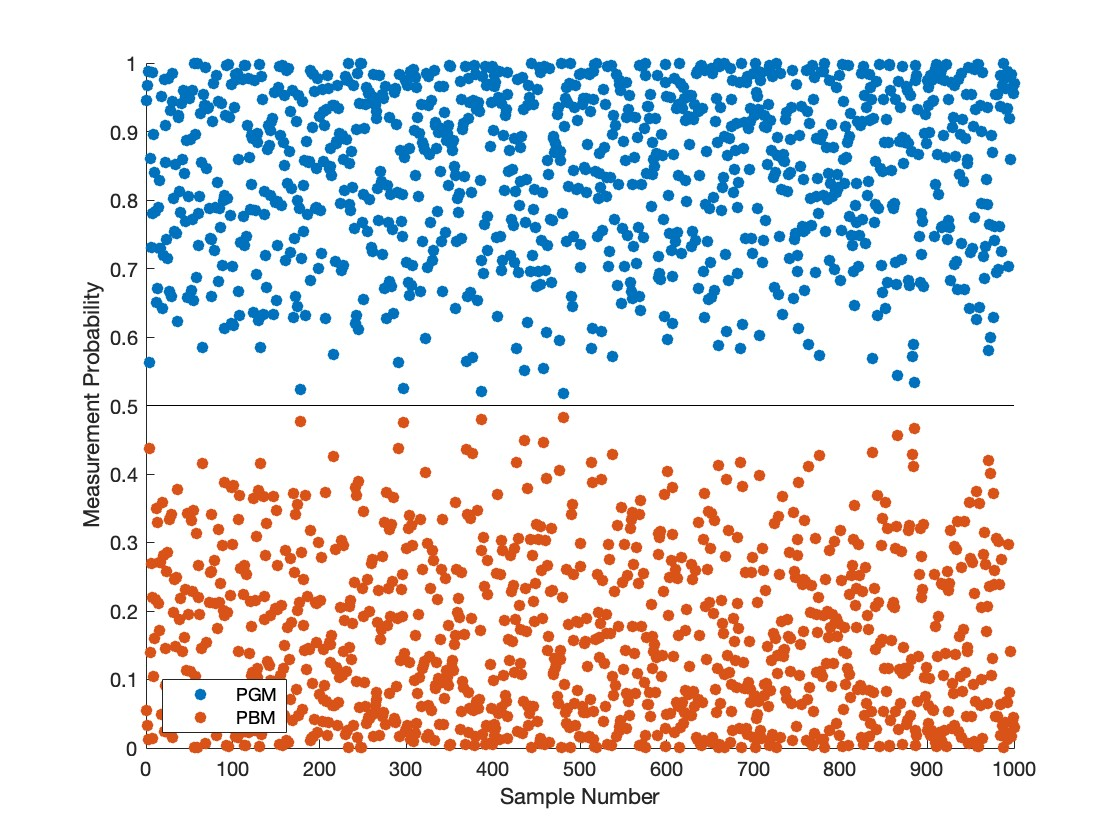
\includegraphics[scale=0.3]{figs/ch4_PBM/pgm_vs_pbm_two_states_rand_probs.jpg}
    \caption{ 
    Computing PGM and PBM for $1000$ instances of $2$ randomly chosen qubits (also with randomly chosen probabilities).  
    Notice that PGM always performs better than $1/2$ and PBM always performs worse than $1/2$. %(although they sometimes get close). 
    }
    \label{fig:ch4_PBM-pgm_vs_pbm_two_states}
\end{figure}
\end{comment}

\begin{figure}[h]
    \centering
    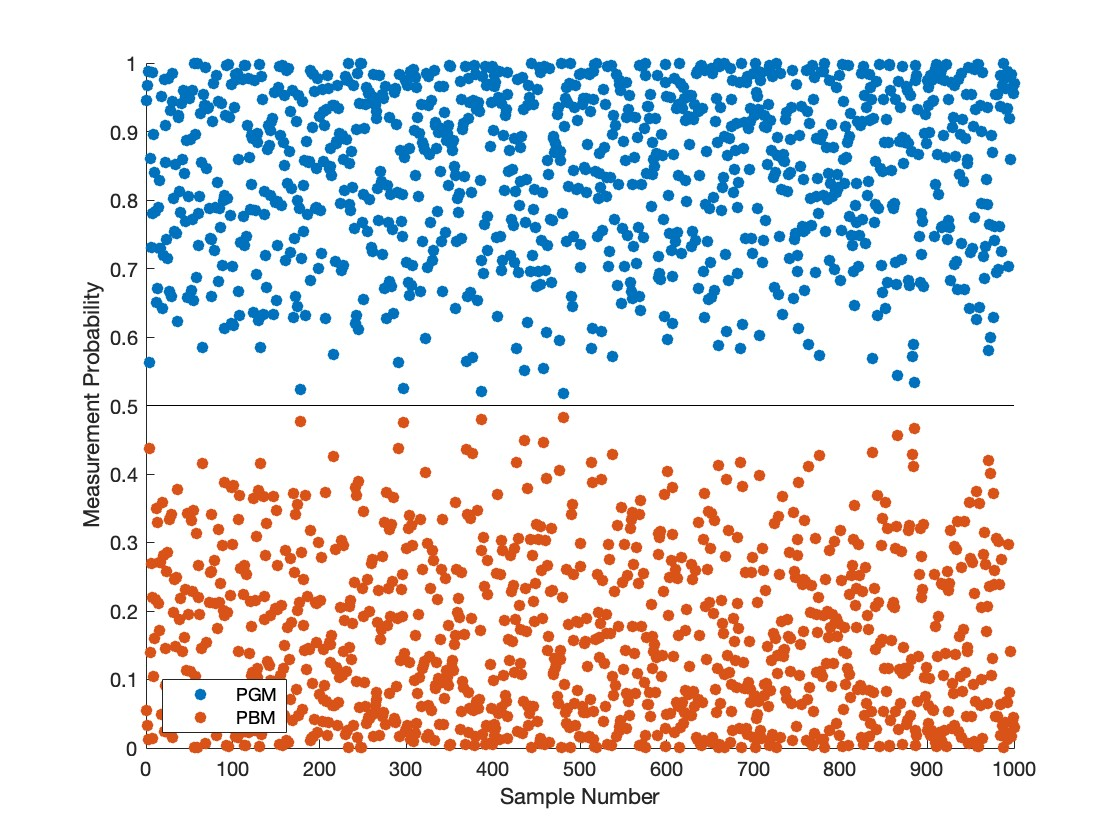
\includegraphics[
        scale=0.3,
        alt={
            Plot comparing the success probabilities of the pretty good measurement and the pretty bad measurement for one thousand randomly generated pairs of qubit states with randomly chosen prior probabilities. 
            Each instance contributes one value for each measurement. 
            Across all instances, the pretty good measurement has success probability greater than one half, while the pretty bad measurement has success probability less than one half.
        }
    ]{figs/ch4_PBM/pgm_vs_pbm_two_states_rand_probs.jpg}

    \caption{
        Success probabilities of the pretty good measurement and pretty bad measurement for 1000 randomly generated pairs of qubit states with randomly chosen prior probabilities. 
        The pretty good measurement always achieves a success probability greater than $1/2$, whereas the pretty bad measurement always achieves a success probability less than $1/2$.
    }
    \label{fig:ch4_PBM-pgm_vs_pbm_two_states}
\end{figure}

\begin{comment}
\begin{figure}[h]
    \centering 
    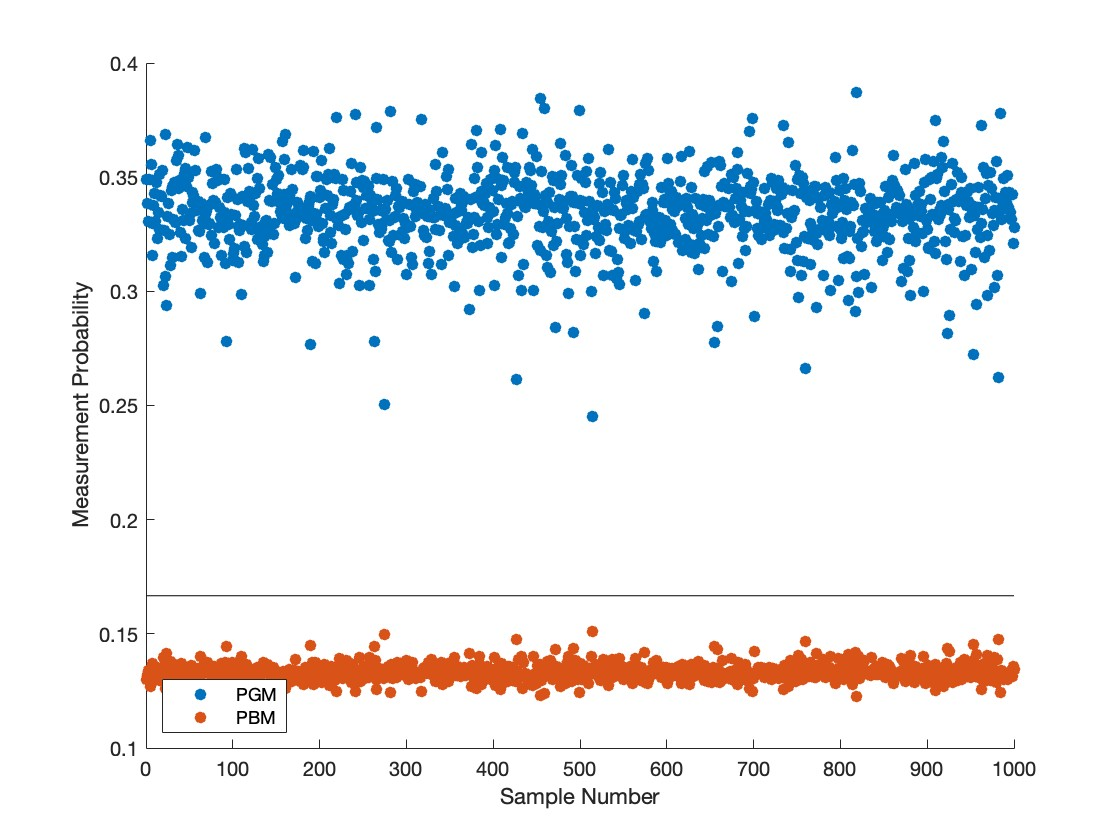
\includegraphics[scale=0.3]{figs/ch4_PBM/pgm_vs_pbm_six_states_rand_probs.jpg}
    \caption{
    Computing PGM and PBM for $1000$ instances of $6$ randomly chosen qubits (also with randomly chosen probabilities).   
        We notice that $\PPGM$ seemingly clusters around $\frac{2}{n}$ and $\PPBM$ seemingly clusters around $\frac{n-2}{n(n-1)}$ for small values of $n$, with $n=6$ illustrated here. 
    } 
    \label{fig:ch4_PBM-pgm_vs_pbm_six_states}
\end{figure} 
\end{comment}

\begin{figure}[h]
    \centering 
    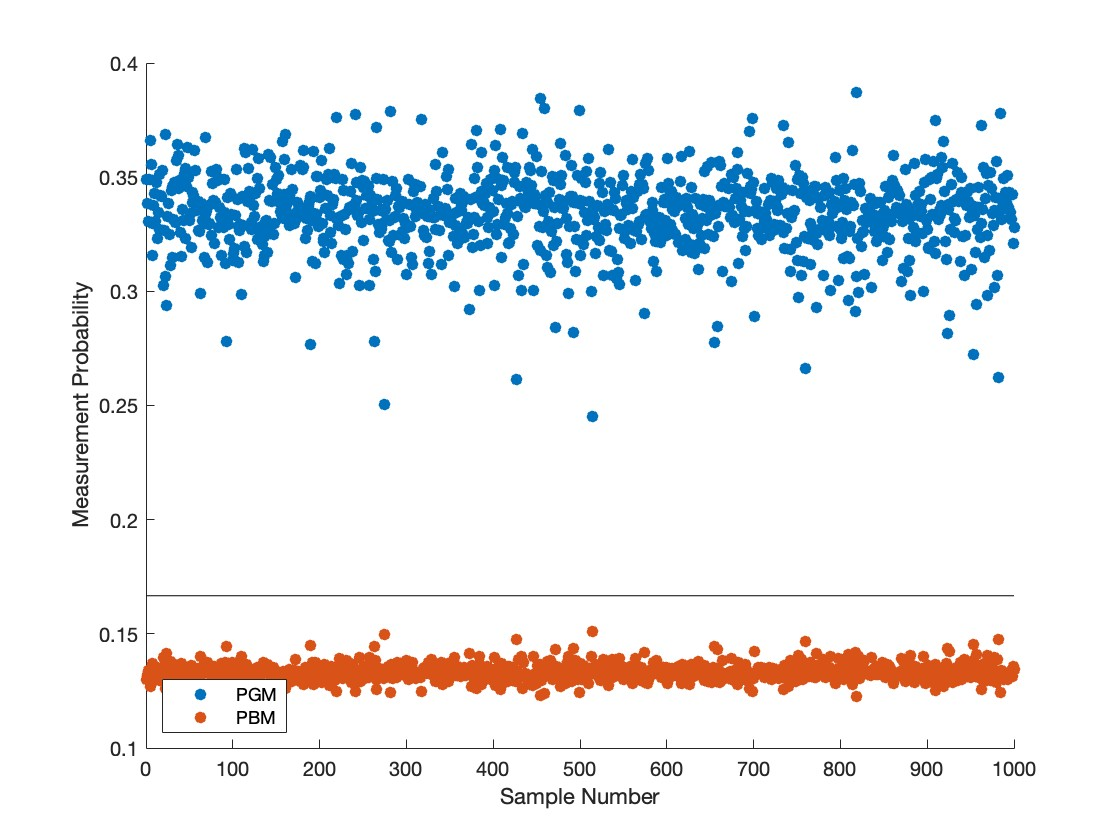
\includegraphics[
        scale=0.3,
        alt={
            Plot comparing the success probabilities of the pretty good measurement and the pretty bad measurement for one thousand randomly generated ensembles. 
            Each ensemble contains six qubit states with randomly selected prior probabilities. 
            The pretty good measurement values cluster near one third, corresponding to two divided by six. 
            The pretty bad measurement values cluster near two fifteenths, corresponding to four divided by thirty.
        }
    ]{figs/ch4_PBM/pgm_vs_pbm_six_states_rand_probs.jpg}

    \caption{
        Success probabilities of the pretty good measurement and pretty bad measurement for 1000 randomly generated ensembles of six qubit states with randomly selected prior probabilities.
        For small values of $n$, $\PPGM$ appears to cluster around $\frac{2}{n}$, while $\PPBM$ appears to cluster around $\frac{n-2}{n(n-1)}$. 
        The case $n=6$ is shown here.
    } 
    \label{fig:ch4_PBM-pgm_vs_pbm_six_states}
\end{figure}

%%%%%%%%%%%%%%%%%%%%%%%%%%%%%%%%%%%%%%%%%%%%%%%%%%%%%%%%%%%%%%%%%%%%%%%%%%%%%%%%%%%%%%%%%%%%%%%%%%%%%%%%%%%%%%%%%%%%%%%%%%%%%%%%%%%
\section{Application: Quantum anomaly detection/avoidance} \label{sec:ch4_PBM-anomaly}
%%%%%%%%%%%%%%%%%%%%%%%%%%%%%%%%%%%%%%%%%%%%%%%%%%%%%%%%%%%%%%%%%%%%%%%%%%%%%%%%%%%%%%%%%%%%%%%%%%%%%%%%%%%%%%%%%%%%%%%%%%%%%%%%%%%

Suppose Alice promises to send Bob $N$ copies of a state $\rho$. 
However, she has a faulty device which is known to produce one copy of an anomaly (read: a \emph{pretty bad state}) $\sigma$ at some point in this sequence. 
Upon receiving the $N$ states, Bob wants to identify a state \emph{which is not faulty}, i.e., not $\sigma$. 

Our approach is to cast this as a discrimination problem with the states 
$$\rho_i = \rho^{\otimes (i-1)}\ \otimes\ \sigma\ \otimes\ \rho^{\otimes (N-i)},$$
for $i \in [N]$, and to use the pretty bad measurement. 
Note that $\rho_i$ is simply $N$ copies of $\rho$, but with $\sigma$ in the $i$-th spot. 
In the traditional discrimination task, Bob is trying to guess where the anomaly has occurred.
However, this is overkill if we just want to find a place where it \emph{did not occur}. 
Thus, taking the perspective of state exclusion makes more sense here. 
In other words, we do want to determine where the anomaly occurred as much as where it \emph{did not occur}. 
We focus on these two concepts in the following example and graphs. 

As an example, we consider the case where Alice promises to send to Bob $7$ copies of the state $\rho = \ketbra{0}{0}$ but an anomaly occurs creating the state $\sigma = \ketbra{\psi}{\psi}$ where $\ket{\psi} = \gamma \ket{0} + \sqrt{1 - \gamma^2} \ket{1}$ for some fixed parameter $\gamma \in [0,1]$ known to both Alice and Bob. 
Fig.~\ref{fig:ch4_PBM-anomaly_7} illustrates the probabilities $\Pbest$, $\PPGM$, $\PPBM$, $\Pworst$ and the blind guessing probability $1/N$, as a function of $\gamma$, below. 
For anomaly detection, \cite{llorens2024quantum, skotiniotis2018identification} showed that PGM is indeed the optimal measurement. Moreover they provide a closed-form expression for the optimal success probability. Therefore, using Eq.~\eqref{eq:ch4_PBM-PGM_PBM} we also have an expression for $\PPBM$.

\begin{comment}
\begin{figure}[h]
    \centering
    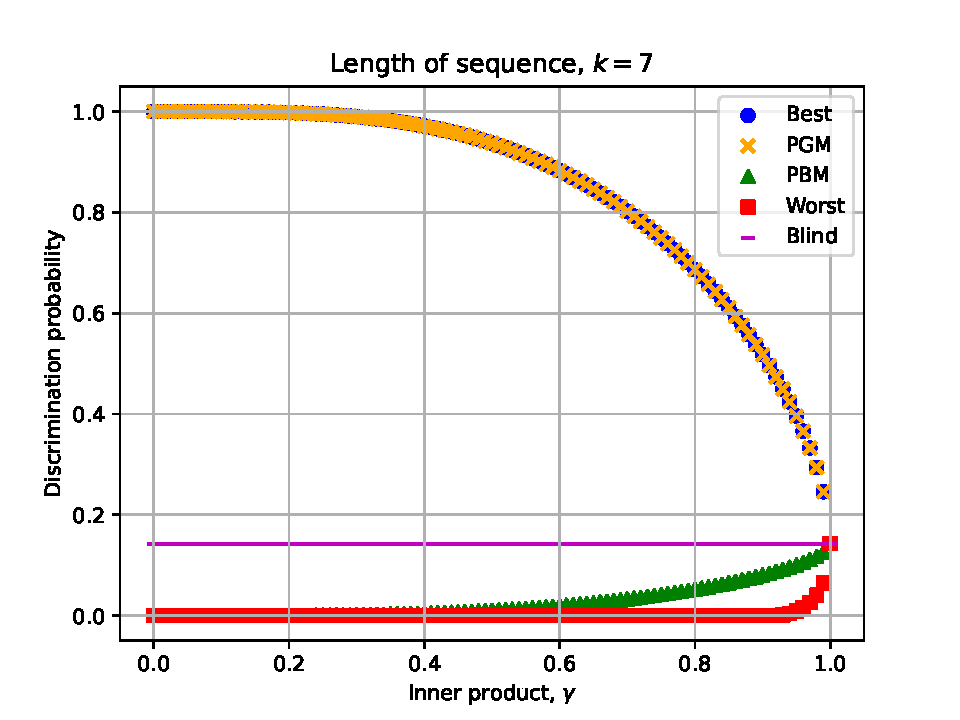
\includegraphics[scale=0.75]{figs/ch4_PBM/anomaly_7-1.pdf}
    \caption{ 
    Probabilities for the quantum state discrimination task defined by the states  
    $\ket{\psi_i} = \ket{0}^{\otimes{i-1}} \otimes \ket{\psi} \otimes \ket{0}^{\otimes{7-i}}$, where $\ket{\psi} = \gamma \ket{0} + \sqrt{1 - \gamma^2} \ket{1}$ and $i \in \{ 1, \ldots, 7 \}$.  
    Observe that while $\PPGM = \Pbest$ for all values of $\gamma$, $\PPBM$ departs from the worst probability around $\gamma = 0.4$. 
    All of these probabilities coincide at $\gamma = 1$ since all the states are the same in this case (see Eq.~(\ref{eq:ch4_PBM-allthesame})).  
    }
    \label{fig:ch4_PBM-anomaly_7}
\end{figure}
\end{comment}

\begin{figure}[h]
    \centering
    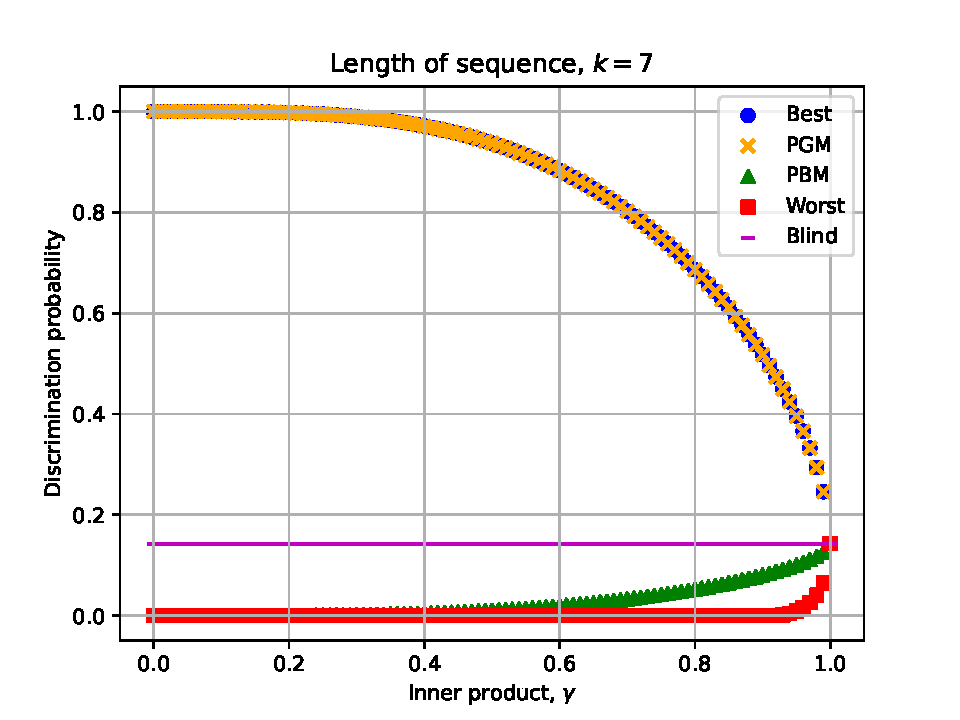
\includegraphics[
        scale=0.75,
        alt={
            Plot comparing four discrimination probabilities for an ensemble of seven quantum states as the overlap parameter gamma varies. 
            Each state contains one anomalous qubit psi at one of seven possible positions, with all other qubits in the zero state. 
            The pretty good measurement probability coincides with the optimal success probability throughout the plotted range. 
            The pretty bad measurement probability initially follows the worst success probability but begins to depart from it near gamma equal to zero point four.
            At gamma equal to one, all four probabilities coincide because the seven states become identical.
        }
    ]{figs/ch4_PBM/anomaly_7-1.pdf}

    \caption{
        Probabilities for the quantum state discrimination task defined by $\ket{\psi_i} = \ket{0}^{\otimes(i-1)} \otimes \ket{\psi} \otimes \ket{0}^{\otimes(7-i)}$, where $\ket{\psi} = \gamma\ket{0} + \sqrt{1-\gamma^2}\ket{1}$ and $i\in\{1,\ldots,7\}$.
        While $\PPGM=\Pbest$ for all values of $\gamma$, $\PPBM$ begins to depart from the worst success probability near $\gamma=0.4$. All four probabilities coincide at $\gamma=1$, since all the states are identical in this case; see Eq.~\eqref{eq:ch4_PBM-allthesame}.
    }
    \label{fig:ch4_PBM-anomaly_7}
\end{figure}

Recall that in the anomaly avoidance problem, we want to identify a state that did not occur. 
Since PBM is trying to minimize $\sum_{i=1}^N \frac{1}{N} \inner{M_i}{\rho_i}$, what PBM is approximating in the context of anomaly avoidance is the minimum average error. 
In this case, the probability of \emph{success} using PBM is $1 - \PPBM$. 
In Fig.~\ref{fig:ch4_PBM-anomaly_7_success}, we compare this probability to that given by PGM which approximates the best average identification probability.  

\begin{comment}
\begin{figure}[h]
    \centering
    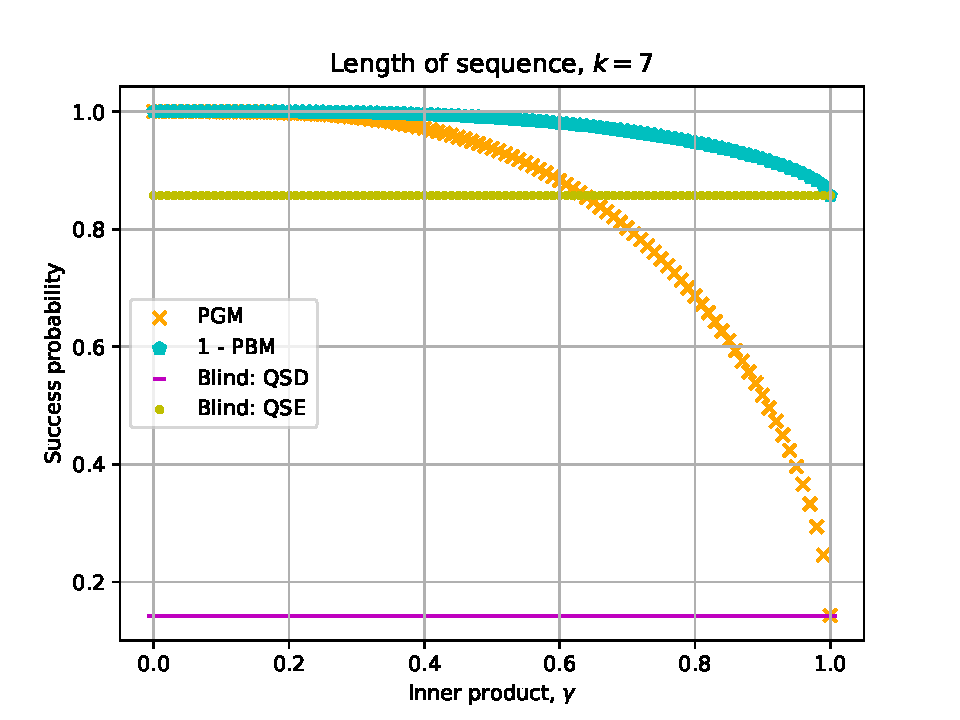
\includegraphics[scale=0.75]{figs/ch4_PBM/anomaly_7_success-3.pdf}
    \caption{ 
    Given one of the states $\ket{\psi_i} = \ket{0}^{\otimes{i-1}} \otimes \ket{\psi} \otimes \ket{0}^{\otimes{7-i}}$, where $\ket{\psi} = \gamma \ket{0} + \sqrt{1 - \gamma^2} \ket{1}$, ranging over $i \in \{ 1, \ldots, 7 \}$, each with equal probability, we plot the probability of successfully avoiding the anomaly $\ket{\psi}$ via PBM and also the probability of successfully identifying $\ket{\psi}$ via PGM. 
    Notice that $\PPGM$ decreases rapidly starting around $\gamma = 0.2$, converging to the blind identification guessing  probability of $1/7$ when $\gamma = 1$. 
    On the other hand, $1 - \PPBM$ decreases at a much slower pace converging to the blind excluding probability of $6/7$ when $\gamma = 1$. 
    We remark that the exclusion probability is much larger than the identification probability, which is to be expected. 
    } 
    \label{fig:ch4_PBM-anomaly_7_success}
\end{figure} 
\end{comment}

\begin{figure}[htbp]
    \centering
    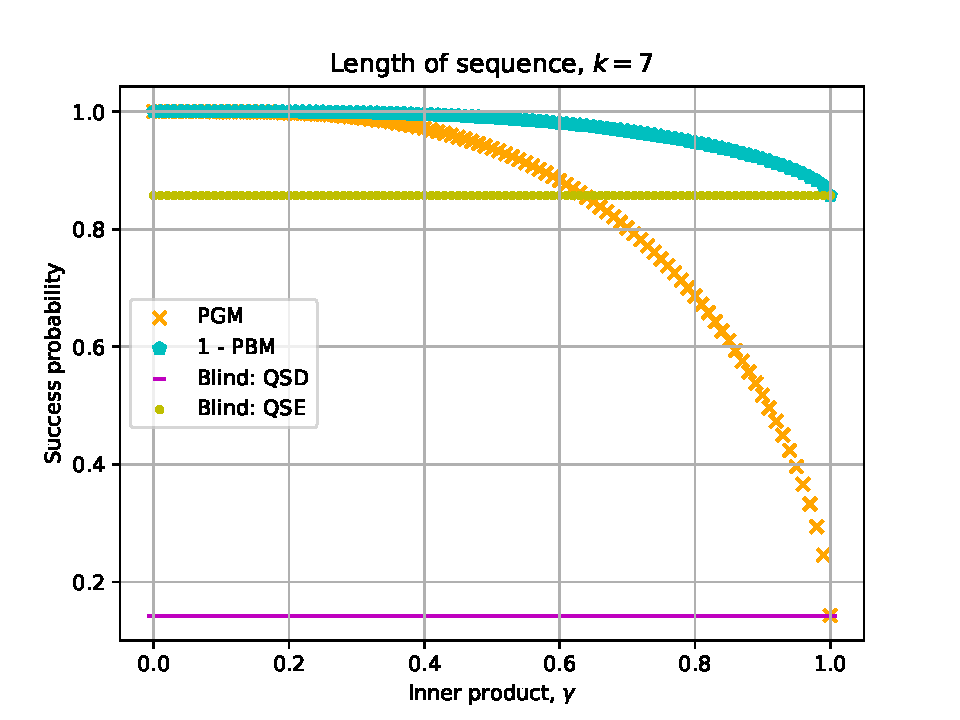
\includegraphics[
        scale=0.75,
        alt={
            Plot comparing identification and exclusion success probabilities for an ensemble of seven equally likely quantum states containing one anomalous qubit. 
            The horizontal axis represents gamma, which controls how similar the anomalous state is to the zero state. 
            The vertical axis represents success probability. 
            The pretty good measurement identification probability decreases rapidly beginning near gamma equal to zero point two and approaches the blind-guessing probability of one seventh at gamma equal to one. 
            The pretty bad measurement exclusion success probability, one minus the pretty bad measurement probability, decreases more slowly and approaches the blind-exclusion probability of six sevenths at gamma equal to one. 
            The exclusion success probability remains substantially greater than the identification success probability.
        }
    ]{figs/ch4_PBM/anomaly_7_success-3.pdf}

    \caption{
        Given one of the equally likely states $\ket{\psi_i} = \ket{0}^{\otimes(i-1)} \otimes \ket{\psi} \otimes \ket{0}^{\otimes(7-i)}$, where $\ket{\psi} = \gamma\ket{0} + \sqrt{1-\gamma^2}\ket{1}$ and $i\in\{1,\ldots,7\}$, we plot the probability of successfully excluding the anomaly $\ket{\psi}$ using the PBM and the probability of successfully identifying $\ket{\psi}$ using the PGM. 
        The probability $\PPGM$ decreases rapidly beginning near $\gamma=0.2$ and approaches the blind identification probability of $1/7$ at $\gamma=1$. 
        In contrast, the exclusion success probability $1-\PPBM$ decreases more slowly and approaches the blind exclusion probability of $6/7$ at $\gamma=1$. 
        As expected, the exclusion success probability is substantially greater than the identification success probability.
    }
    \label{fig:ch4_PBM-anomaly_7_success}
\end{figure}

\begin{comment}
\medskip 
\paragraph{Conclusions.} 
In this work we introduced the pretty bad measurement as a means to approximate the worst guessing probability for quantum state discrimination and compared it to the pretty good measurement. 
We showed that they have an intricate relationship and proved that each compare favorably to simply randomly guessing. 
Finally, we examined the quantum anomaly detection/avoidance problem and gave an illustrative example showing how these measurements perform for detecting/avoiding parameterized quantum states. 

\medskip 
\paragraph{Acknowledgements.} 
The authors thank Iman Marvian, Vincent Russo, Nathaniel Johnston, and Santiago Llorens for useful discussions. 
This research was funded in part by the Commonwealth of Virginia’s Commonwealth Cyber Initiative (CCI) under grant number~{467714}. 

%\bibliographystyle{alpha}
%\bibliography{PBM_arxiv_v2}

%\appendix  
\end{comment}


